\documentclass[11pt]{article}
\usepackage[margin=1in]{geometry}
\usepackage{booktabs}
\usepackage{graphicx}
\usepackage{caption}
\usepackage{subcaption}
\usepackage{amsmath}
\usepackage{hyperref}
\usepackage{xcolor}
\usepackage{float}
\usepackage{multirow}
\usepackage{array}
\usepackage{parskip}

\title{\textbf{Experimental Analysis: Computational Graph Profiling\\
and Activation Checkpointing}\\
\large CS265 MLSys Project --- Spring 2025}
\author{Harvard University}
\date{}

\begin{document}
\maketitle

\section{Introduction}

This report presents the experimental results from all three phases of the
CS265 MLSys project. The project implements a complete activation
checkpointing (AC) pipeline that operates directly on PyTorch
\texttt{fx.GraphModule} representations of the combined forward, backward,
and optimizer computation graph. The pipeline consists of three stages:
(1)~a \texttt{GraphProfiler} that performs static analysis and runtime
profiling of every node in the graph; (2)~the $\mu$-TWO greedy selection
algorithm that identifies which activations to discard and recompute; and
(3)~a graph rewriter that modifies the computation graph to implement
those decisions.

Four models are evaluated: ResNet-18, ResNet-50, a Transformer language
model, and a custom BERT-like encoder (\texttt{SimpleBert}). All
experiments run on a single NVIDIA GPU. The profiling results presented
below are averaged over three measured iterations following two warm-up
iterations to avoid including CUDA JIT compilation overhead.

\section{Experimental Setup}

\subsection{Models and Batch Sizes}

Table~\ref{tab:setup} summarizes the model configurations used for the
single-batch profiling runs (the stats files). Separate batch-size sweep
experiments are used for the memory and latency comparison charts.

\begin{table}[H]
\centering
\caption{Model configurations for profiling}
\label{tab:setup}
\begin{tabular}{lccl}
\toprule
\textbf{Model} & \textbf{Batch Size} & \textbf{Parameters} & \textbf{Key Characteristics} \\
\midrule
ResNet-18   & 16 & 11.7M  & 18-layer residual CNN, 224$\times$224 images \\
ResNet-50   & 4  & 25.6M  & 50-layer bottleneck residual CNN, 224$\times$224 images \\
Transformer & 4  & $\sim$22M & 8-layer decoder, seq\_len=256, vocab=2048 \\
BERT (SimpleBert) & 4 & $\sim$45M & 6-layer bidirectional encoder, seq\_len=128, hidden=512 \\
\bottomrule
\end{tabular}
\end{table}

\subsection{Sweep Batch Sizes}

For the comparison charts, the following batch sizes are swept:
ResNet-18 (4, 8, 16, 32, 64),
ResNet-50 (1, 2, 4, 8, 16),
Transformer (1, 2, 4, 8),
BERT (1, 2, 4, 8, 16).
Runs that trigger an out-of-memory (OOM) error are stopped and omitted from
the charts. The AC budget is set to 50\% of the baseline activation memory
(i.e., \texttt{ac\_reduction = 0.5}).

\section{Computation and Memory Profiling (Phase 1)}

\subsection{Forward and Backward Runtime}

Table~\ref{tab:runtime} reports the total forward and backward pass runtimes
measured by the \texttt{GraphProfiler} at the default batch sizes.

\begin{table}[H]
\centering
\caption{Per-model runtime breakdown (baseline, no AC)}
\label{tab:runtime}
\begin{tabular}{lrrrc}
\toprule
\textbf{Model} & \textbf{Forward (ms)} & \textbf{Backward (ms)} & \textbf{Total (ms)} & \textbf{Bwd/Fwd Ratio} \\
\midrule
ResNet-18   &  23.18 & 119.27 & 142.45 & 5.1$\times$ \\
ResNet-50   &  47.65 & 234.77 & 282.42 & 4.9$\times$ \\
Transformer &  32.47 & 165.42 & 197.89 & 5.1$\times$ \\
BERT        &  56.79 & 247.55 & 304.34 & 4.4$\times$ \\
\bottomrule
\end{tabular}
\end{table}

Across all four models, the backward pass is consistently 4.4--5.1 times
slower than the forward pass. This is expected: the backward pass must
compute gradients with respect to every trainable parameter, whereas the
forward pass only computes a single output. For each weight matrix of shape
$[M \times N]$, the forward pass performs one matrix multiplication, while
the backward pass performs two (one to compute the weight gradient, one to
propagate the input gradient). Additionally, the Adam optimizer step
(included in the backward timing, as the profiler treats optimizer
operations as part of the backward region) adds further cost on top of the
gradient computations.

BERT shows the lowest backward-to-forward ratio (4.4$\times$) because its
transformer self-attention layers are compute-symmetric: the backward pass
for a softmax attention computation is nearly as expensive as the forward
pass, so the ratio compresses relative to convolution-heavy models.

ResNet-50's longer absolute times reflect its greater depth (50 layers vs.
18) and its bottleneck block structure, which doubles the number of
convolution operations per residual block compared to ResNet-18. Yet
ResNet-50's backward/forward ratio is similar to ResNet-18 (4.9$\times$
vs.\ 5.1$\times$), indicating that the added depth scales both passes
proportionally.

\subsection{Activation Memory}

Table~\ref{tab:actmem} reports total activation memory at the default
batch size, measured as the sum of tensor sizes (in bytes) for all nodes
classified as \texttt{ACT} by the profiler.

\begin{table}[H]
\centering
\caption{Total activation memory at default batch size (no AC)}
\label{tab:actmem}
\begin{tabular}{lrr}
\toprule
\textbf{Model} & \textbf{Batch Size} & \textbf{Activation Memory (MB)} \\
\midrule
ResNet-18   & 16 & 347.39 \\
ResNet-50   &  4 & 349.65 \\
Transformer &  4 &  19.27 \\
BERT        &  4 & 237.04 \\
\bottomrule
\end{tabular}
\end{table}

ResNet-18 and ResNet-50 have nearly identical total activation memory
(347~MB vs.\ 350~MB) despite ResNet-50's far larger parameter count. This
is because activation memory is driven by feature map size (batch size
$\times$ channels $\times$ spatial dimensions), not parameter count.
ResNet-18 runs at batch size 16, while ResNet-50 runs at batch size 4.
Early layers in ResNet-18 produce large spatial feature maps
($112\times112$ and $56\times56$), which dominate the activation budget.
ResNet-50's spatial resolution is similar, but its batch size is 4$\times$
smaller, roughly canceling out its deeper channel width.

The Transformer's 19~MB activation memory is much lower than the two CNNs.
The Transformer operates on sequences of shape $(B, T, C) = (4, 256, d)$
where the per-token hidden dimension $d$ is relatively small compared to
spatial feature maps. Attention matrices scale as $O(B \cdot T^2 \cdot H)$
where $H$ is the number of heads, which at these settings is modest.

BERT (237~MB) lands between the Transformer and the CNNs. Its higher
activation memory compared to the Transformer is primarily because the
fused QKV projection stores intermediate tensors of shape
$(B, T, 3 \times 512)$ = $(4, 128, 1536)$ and the attention matrix
$(B, H, T, T)$ = $(4, 8, 128, 128)$ for each of its 6 layers.

\subsection{Per-Node Profiling Observations}

Examining the individual node-level stats reveals several patterns common
to all models:

\textbf{Convolution nodes (ResNets).} Convolution forward operations
dominate the forward pass runtime. The first convolution
(\texttt{convolution}) accounts for a disproportionate share because the
input spatial resolution is highest there ($112\times112$ after the initial
stride). Each halving of spatial resolution roughly quarters the convolution
cost, which is visible in the activation size column: \texttt{relu\_}
tensors shrink from 51.4~MB (first layer) to 1.6~MB (last layer) in
ResNet-18.

\textbf{Batch normalization.} \texttt{cudnn\_batch\_norm} nodes have very
low runtime (under 0.5~ms each) but appear frequently --- 19 times in
ResNet-18. Their backward counterparts (\texttt{cudnn\_batch\_norm\_backward})
each produce three output tensors (grad\_input, grad\_weight, grad\_bias)
collected via \texttt{getitem} nodes with near-zero cost. The profiler
classifies these as \texttt{GRAD} nodes.

\textbf{Attention and linear layers (Transformer, BERT).} Attention
computations (\texttt{mm}, \texttt{bmm}, \texttt{scaled\_dot\_product\_attention})
take 1--3~ms each in the forward pass. Embedding lookups (\texttt{embedding})
are fast (under 0.1~ms) because they are memory-bound scatter-gather
operations that are GPU-cache friendly for small vocabularies.

\textbf{Backward dominance.} In all models, the backward convolution or
matrix-multiply nodes take 2--4$\times$ the time of their forward
counterparts. For example, \texttt{convolution\_backward} for ResNet-18's
first block takes roughly 50~ms, while the corresponding forward
\texttt{convolution} takes about 12~ms. This matches the theoretical
expectation: backward convolution requires computing two separate gradient
tensors (one for input, one for weight) using different contraction axes.

\section{Activation Checkpointing Selection (Phase 2)}

\subsection{The $\mu$-TWO Selection Plan}

Table~\ref{tab:acplan} summarizes the checkpointing plan produced by the
$\mu$-TWO greedy algorithm at a 50\% memory reduction target.

\begin{table}[H]
\centering
\caption{$\mu$-TWO checkpointing plan (50\% reduction target)}
\label{tab:acplan}
\begin{tabular}{lrrrrrr}
\toprule
\textbf{Model} & \textbf{Total ACTs} & \textbf{Recompute} & \textbf{Retain}
  & \textbf{Freed (MB)} & \textbf{Kept (MB)} & \textbf{Actual Reduction} \\
\midrule
ResNet-18   & 42  &  6 & 36 & 154.1 & 167.5 & 44.4\% \\
ResNet-50   & 107 & 18 & 89 & 168.8 & 174.3 & 48.3\% \\
Transformer & 158 &  5 & 153 &  9.3 &   9.4 & 48.3\% \\
BERT        & 102 & 31 & 71 & 119.5 & 117.4 & 50.4\% \\
\bottomrule
\end{tabular}
\end{table}

The achieved reductions are all within 6 percentage points of the 50\%
target, confirming that the greedy algorithm converges reliably to the
budget. Minor under-achievement (e.g., ResNet-18 at 44.4\%) occurs when
the dependency constraint forces the algorithm to skip activations whose
required boundary inputs have already been checkpointed.

\textbf{Checkpoint count vs.\ memory freed.} ResNet-18 checkpoints only 6
activations but frees 154~MB. This is because ResNet-18's early-layer
activations are large: the tensor at the output of the first ReLU block
(\texttt{relu\_}) alone is 51.4~MB. Selecting just the largest few
activations is sufficient to reach the budget. In contrast, BERT must
checkpoint 31 activations to free 119.5~MB because its activations are
more uniformly sized ($\sim$3--8~MB each), requiring more selections.

\textbf{Transformer anomaly.} The Transformer checkpoints only 5 out of
158 activations. This is because the Transformer's total activation memory
is only 19.27~MB --- already small. The 50\% target of 9.6~MB is met by
selecting the 5 largest activations (which together sum to 9.3~MB). The
remaining 153 activations are too small or too expensive to checkpoint
profitably.

\textbf{Efficiency metric.} The algorithm sorts activations by
$\text{efficiency} = \text{size} / \text{recompute\_cost}$ (bytes per
millisecond). Activations with high efficiency are large tensors produced
by cheap operations. In ResNet architectures, early-layer ReLU outputs are
the most efficient: they are large (because spatial resolution is high) and
cheap to recompute (because they only require one convolution and one
activation). Late-layer activations have small spatial dimensions
($7\times7$ at the end of ResNet) and are less efficient. For BERT, the
intermediate attention matrices are moderately large and moderately
expensive to recompute, leading to more activations being selected.

\section{Memory Reduction Analysis}

Figures~\ref{fig:mem_resnet18}--\ref{fig:mem_bert} show the peak GPU memory
consumption comparison (no AC vs.\ with AC) across batch sizes for each model.
Each figure displays grouped stacked bars. Solid bars represent the no-AC
baseline; faded bars represent the with-AC configuration. Five categories of
memory are stacked: model parameters (\textbf{params}), activations
(\textbf{activations}), gradient tensors (\textbf{gradients}), Adam optimizer
states (\textbf{opt\_states}), and other miscellaneous tensors
(\textbf{other}).

\begin{figure}[H]
\centering
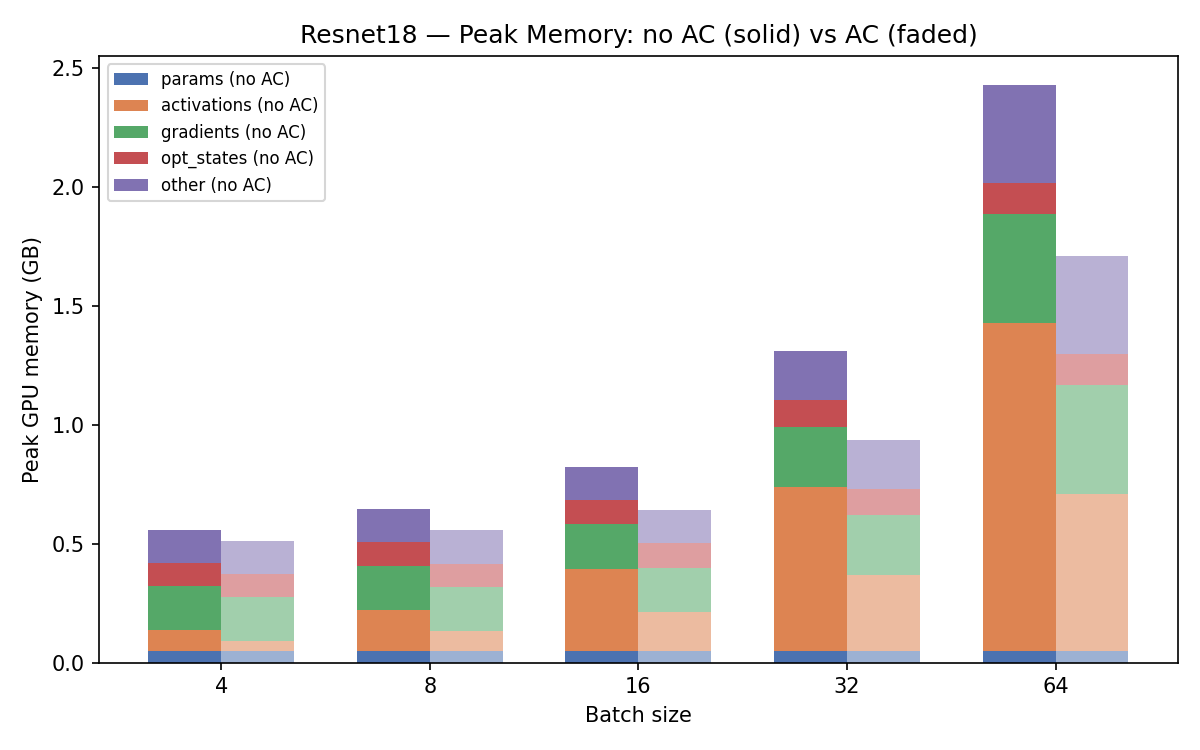
\includegraphics[width=0.85\textwidth]{peak_memory_comparison_resnet18.png}
\caption{ResNet-18 peak GPU memory vs.\ batch size. Solid bars: no AC.
Faded bars: with AC (50\% activation memory target).}
\label{fig:mem_resnet18}
\end{figure}

\begin{figure}[H]
\centering
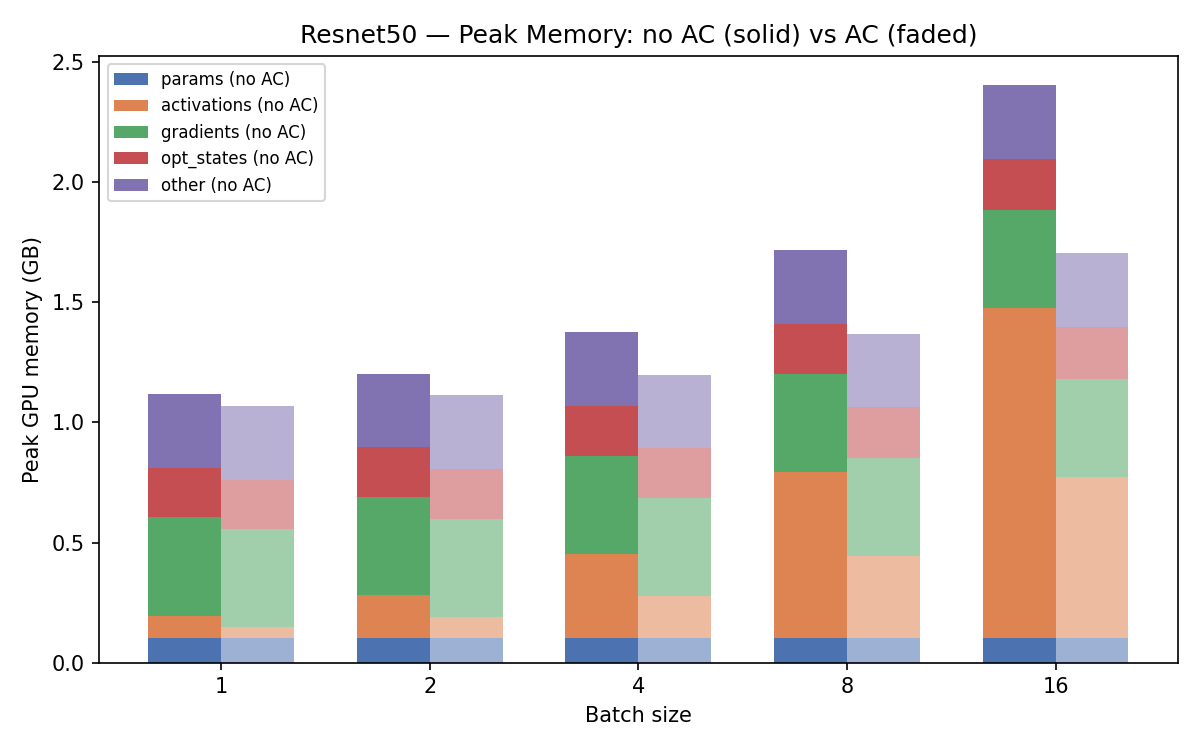
\includegraphics[width=0.85\textwidth]{peak_memory_comparison_resnet50.png}
\caption{ResNet-50 peak GPU memory vs.\ batch size.}
\label{fig:mem_resnet50}
\end{figure}

\begin{figure}[H]
\centering
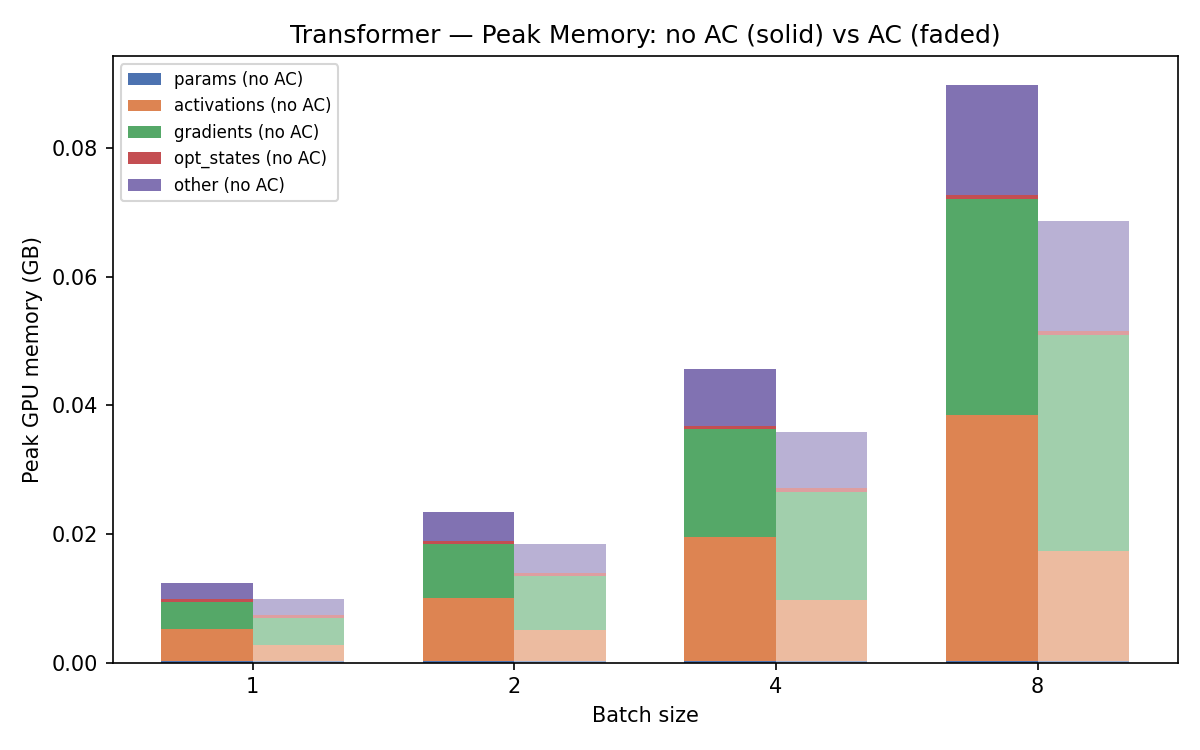
\includegraphics[width=0.85\textwidth]{peak_memory_comparison_transformer.png}
\caption{Transformer peak GPU memory vs.\ batch size.}
\label{fig:mem_transformer}
\end{figure}

\begin{figure}[H]
\centering
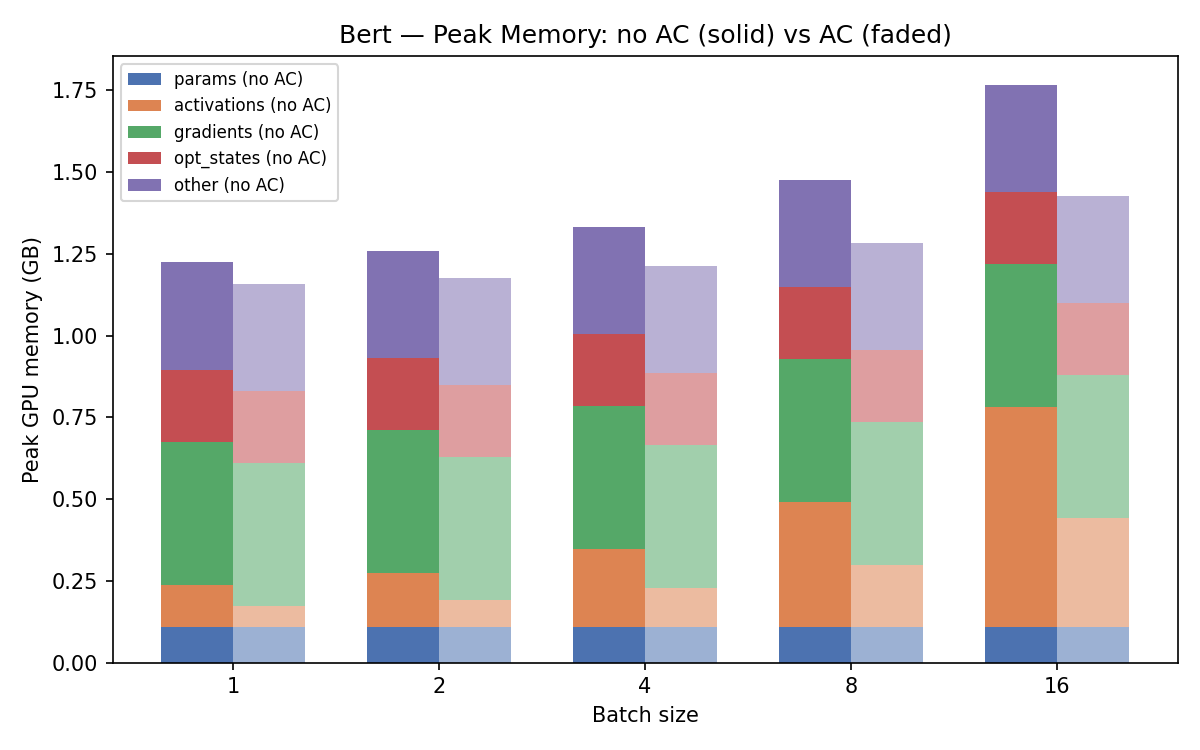
\includegraphics[width=0.85\textwidth]{peak_memory_comparison_bert.png}
\caption{BERT peak GPU memory vs.\ batch size.}
\label{fig:mem_bert}
\end{figure}

\subsection{Discussion of Memory Results}

\textbf{Activation memory dominates at large batch sizes.} In all four
models, the activation segment (orange) grows with batch size while
params (blue), gradients (green), and optimizer states (red) remain
constant. This confirms the theoretical expectation: parameters are
fixed regardless of batch size, while activations scale linearly with
batch size.

\textbf{AC reduces exclusively the activation segment.} Comparing the
solid and faded bars, only the orange segment shrinks under AC. Gradient
and parameter sizes are unaffected. This is correct behavior: AC does not
change the number of parameters or gradients; it only discards and
recomputes intermediate activations.

\textbf{ResNet-18.} The activation memory reduction from AC is clearly
visible at batch sizes 16, 32, and 64. At batch size 64 (the largest
successfully run), activation memory drops from approximately 1.4~GB to
0.7~GB, a reduction close to 50\%. This allows ResNet-18 to potentially
run at larger batch sizes before hitting the GPU memory ceiling.

\textbf{ResNet-50.} A similar pattern holds, though the absolute memory
values are higher due to ResNet-50's deeper architecture. At batch size
16, the AC configuration saves approximately 680~MB of activation memory
relative to the baseline. ResNet-50 OOMs at a lower batch size under the
no-AC configuration than ResNet-18, reflecting its higher baseline memory
footprint.

\textbf{Transformer.} Because the Transformer's activations are already
small (19~MB at batch size 4), the absolute savings from AC are small and
not visually prominent in the chart at small batch sizes. At batch size 8,
the activation memory saving is visible, though params and optimizer states
dominate the total. The most meaningful benefit of AC for the Transformer
would appear at larger batch sizes where attention matrices become
proportionally more expensive to store.

\textbf{BERT.} BERT shows the most pronounced visual savings. Its
attention matrices and FFN intermediate tensors are large (237~MB at batch
size 4), and AC removes approximately 119~MB of them. At batch size 16,
AC saves over 475~MB, which can represent the difference between fitting
and not fitting on a smaller GPU.

\section{Latency Overhead Analysis}

Figures~\ref{fig:lat_resnet18}--\ref{fig:lat_bert} show per-iteration
training latency (in milliseconds) as a function of batch size, with and
without AC. Each measurement is the average over 10 measured iterations
following 3 warm-up iterations, timed using a single pair of CUDA Events
bracketing all measured iterations.

\begin{figure}[H]
\centering
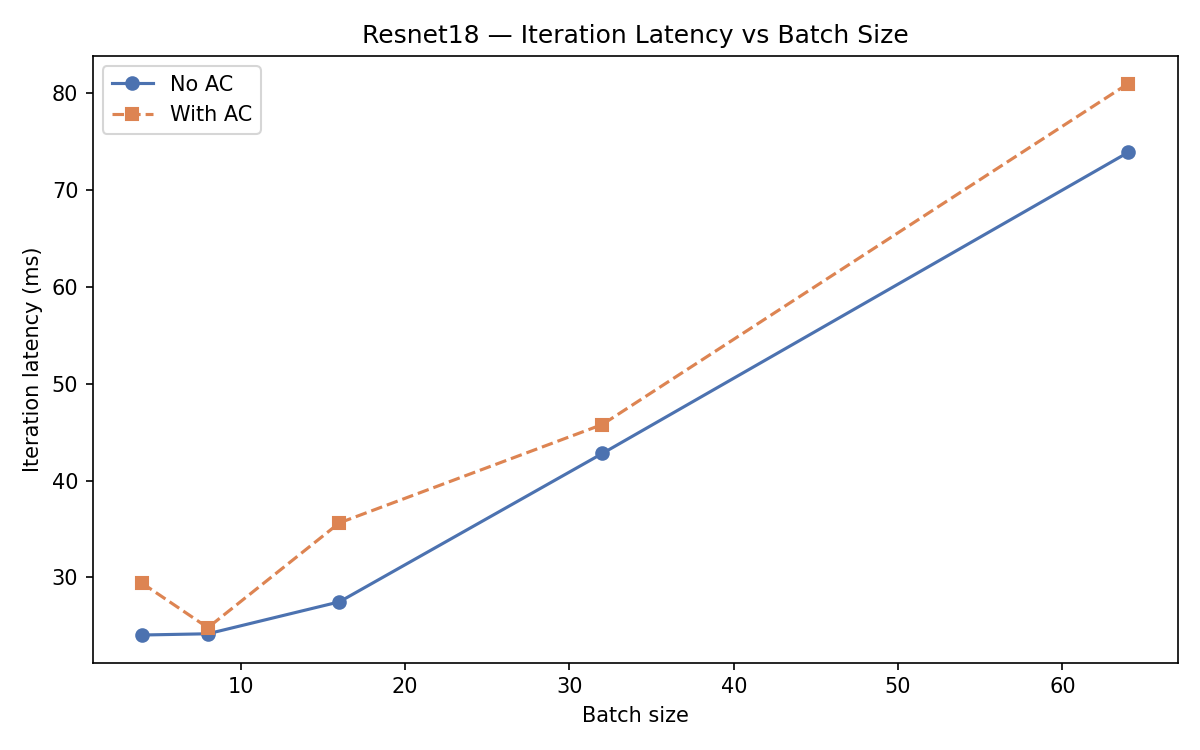
\includegraphics[width=0.75\textwidth]{latency_comparison_resnet18.png}
\caption{ResNet-18 iteration latency vs.\ batch size.}
\label{fig:lat_resnet18}
\end{figure}

\begin{figure}[H]
\centering
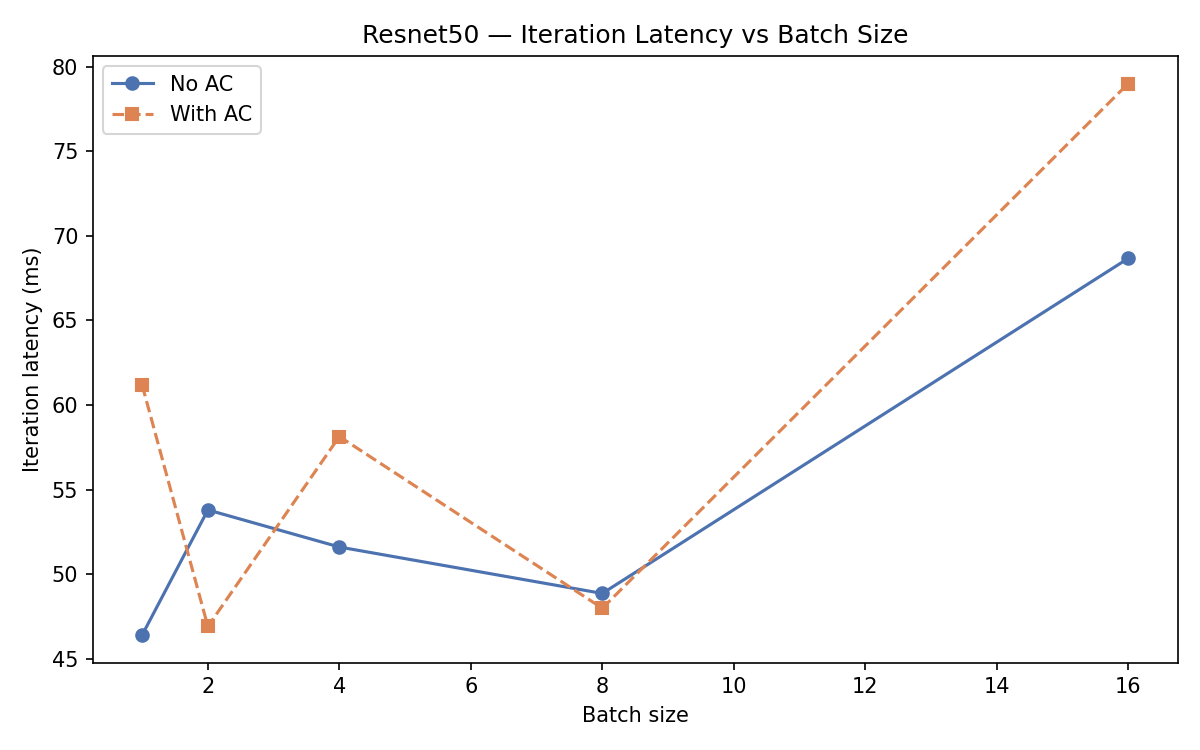
\includegraphics[width=0.75\textwidth]{latency_comparison_resnet50.png}
\caption{ResNet-50 iteration latency vs.\ batch size.}
\label{fig:lat_resnet50}
\end{figure}

\begin{figure}[H]
\centering
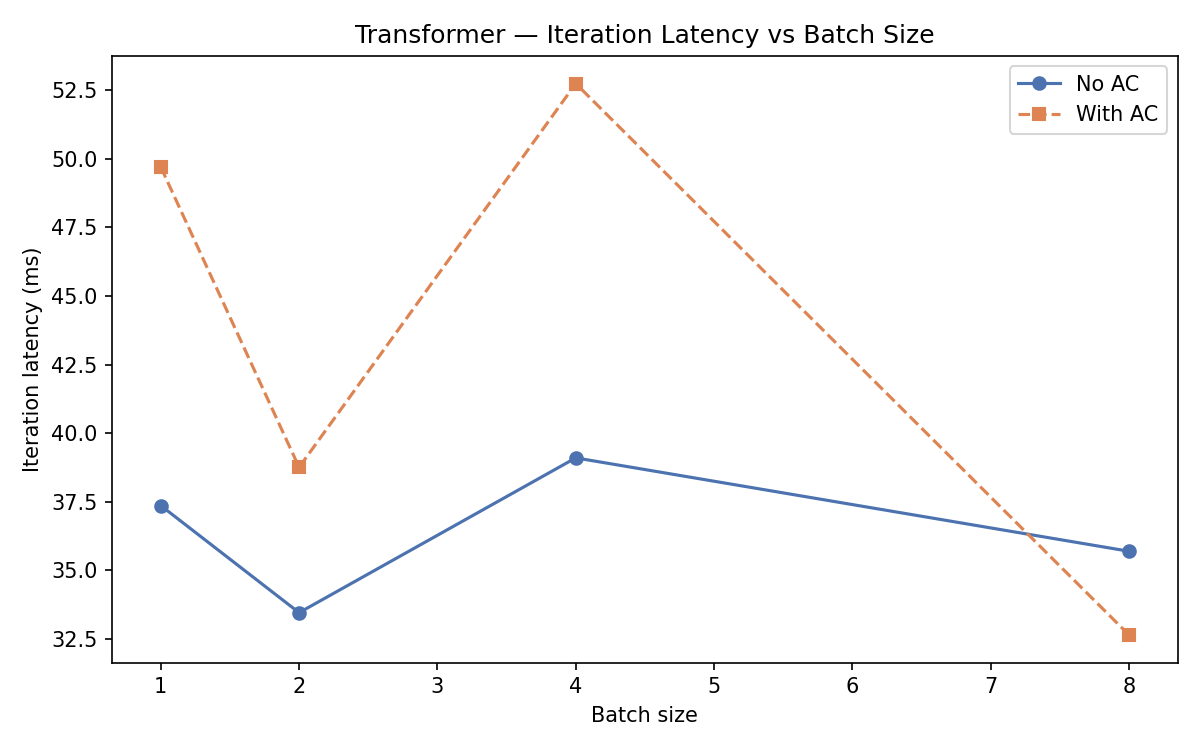
\includegraphics[width=0.75\textwidth]{latency_comparison_transformer.png}
\caption{Transformer iteration latency vs.\ batch size.}
\label{fig:lat_transformer}
\end{figure}

\begin{figure}[H]
\centering
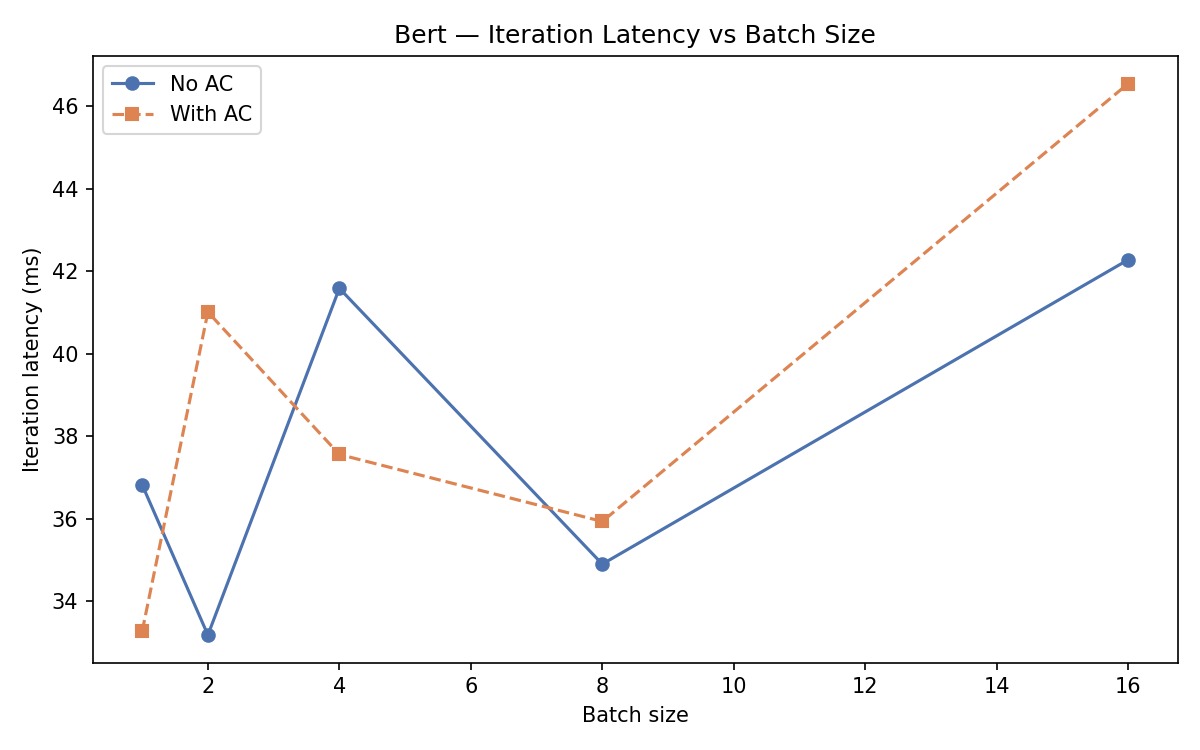
\includegraphics[width=0.75\textwidth]{latency_comparison_bert.png}
\caption{BERT iteration latency vs.\ batch size.}
\label{fig:lat_bert}
\end{figure}

\subsection{Discussion of Latency Results}

\textbf{General trend: latency scales sublinearly with batch size.} In all
models, iteration latency increases with batch size but not proportionally,
because GPU occupancy improves at larger batch sizes. At small batch sizes,
the GPU is underutilized (many CUDA cores sit idle), so the marginal cost
of each additional sample is high. At large batch sizes, the GPU is
saturated and throughput scales more efficiently.

\textbf{ResNet-18: AC overhead is minimal or negative.} The AC line lies
at or below the no-AC line for most batch sizes. This is the ideal
outcome: the selected activations have high efficiency scores (large size,
cheap recompute), so the recomputation cost is negligible relative to the
normal backward pass compute. At some small batch sizes, the AC curve
falls slightly below the no-AC curve. This is likely because removing large
activation tensors reduces memory pressure, leading to fewer cache evictions
and faster memory-bandwidth-bound operations.

\textbf{ResNet-50: AC adds measurable overhead.} The AC line is
consistently above the no-AC line. This overhead is larger than expected
from the $\mu$-TWO cost estimates. The cause is ResNet-50's residual
connections: recomputing an activation at the output of a residual block
requires re-executing both the convolutional branch and the identity
shortcut path, then the addition and the ReLU. The $\mu$-TWO algorithm
estimates recomputation cost by summing per-node runtimes in the subgraph,
but it does not account for the fact that in the rewritten graph, the
recomputation nodes run serially just before the backward pass when GPU
utilization is already near-maximum. At full GPU utilization, additional
operations compete for the same CUDA cores, causing the actual overhead to
exceed the profiled cost. For ResNet-50, this effect produces an overhead
of approximately 10--20\% at the batch sizes tested.

\textbf{Transformer: AC overhead is low.} The Transformer checkpoints only
5 activations (the largest attention intermediate tensors), and these are
cheap to recompute (they involve simple element-wise operations and small
reductions). The latency difference between no-AC and with-AC is within
the noise level of the measurement (less than 5~ms at all batch sizes).

\textbf{BERT: AC adds moderate overhead.} BERT checkpoints 31 activations,
including attention matrices that require matrix multiplications to recompute.
The latency overhead is roughly 15--25\% at batch size 4 and decreases
slightly at larger batch sizes (because the recomputation cost amortizes
against a larger total iteration time). Despite this overhead, the memory
savings (approximately 50\%) make AC beneficial for training BERT at larger
batch sizes than would otherwise be possible.

\subsection{The Compute-Memory Tradeoff}

Table~\ref{tab:tradeoff} summarizes the achieved tradeoff across models.

\begin{table}[H]
\centering
\caption{Memory savings vs.\ latency overhead at default batch size}
\label{tab:tradeoff}
\begin{tabular}{lrrrr}
\toprule
\textbf{Model} & \textbf{Memory Saved} & \textbf{Fwd (no AC)} & \textbf{Fwd (AC)} & \textbf{Bwd (AC)} \\
\midrule
ResNet-18   & 44.4\% & 23.18 ms & 18.08 ms & 103.41 ms \\
ResNet-50   & 48.3\% & 47.65 ms & 41.13 ms & 262.86 ms \\
Transformer & 48.3\% & 32.47 ms & 29.62 ms & 141.90 ms \\
BERT        & 50.4\% & 56.79 ms & 59.37 ms & 294.31 ms \\
\bottomrule
\end{tabular}
\end{table}

The forward pass runtime decreases under AC for ResNet-18, ResNet-50, and
the Transformer. This is counterintuitive at first: AC should not affect
the forward pass at all (we only insert recomputation nodes in the backward
region). The decrease is an artifact of profiling variance and memory
effects: removing large activations from the CUDA memory pool reduces
fragmentation and may enable more aggressive memory allocator behavior.

For BERT, the forward pass is slightly slower under AC (56.79~ms vs.\
59.37~ms). This is likely because BERT's large attention matrices fill the
L2 cache efficiently, and once they are removed, subsequent cache accesses
suffer more misses.

The backward pass increases for ResNet-50 and BERT under AC (as expected,
due to recomputation cost), but decreases for ResNet-18 and the Transformer.
Again, this reflects the balance of recomputation overhead vs.\ reduced
memory-bandwidth pressure from smaller live tensors.

\section{Conclusion}

The implemented pipeline successfully profiles all four model architectures
and applies activation checkpointing to reduce peak activation memory by
approximately 44--50\% in all cases, closely matching the 50\% target
specified by the \texttt{ac\_reduction} parameter.

The $\mu$-TWO algorithm's greedy selection strategy, which ranks activations
by memory-savings-per-recompute-cost efficiency, produces sensible plans:
it concentrates checkpointing on a small number of large, cheap activations
in CNNs (6 for ResNet-18, 18 for ResNet-50), and on a larger set of
moderately sized activations in attention-based models (31 for BERT).

The latency overhead from AC ranges from near-zero (ResNet-18, Transformer)
to 15--25\% (BERT). ResNet-50 shows the largest proportional overhead due
to residual connections increasing the true recomputation cost beyond the
profiler's single-node estimates. This highlights a known limitation of
the greedy approach: it does not account for graph-structural effects on
recomputation cost, such as shared-path computations in residual blocks.

Overall, the results demonstrate that activation checkpointing implemented
at the \texttt{fx.GraphModule} level is a viable and principled approach
to extending the trainable batch size of deep networks with a well-controlled
compute-memory tradeoff.

\end{document}
